\documentclass[journal]{IEEEtran}
\usepackage[T1]{fontenc}
\usepackage[utf8]{inputenc}
\usepackage{amsmath,amssymb,graphicx,booktabs,array,microtype}
\usepackage{float}
\usepackage[hidelinks]{hyperref}
\usepackage{url}
\hypersetup{pdftitle={HyCADO for Detector-Guided Region Refinement in UAV Object Detection},pdfauthor={Gul Erten and Mehmet Koc},pdfsubject={Controlled evaluation of crop placement, resolution, and false-positive budgets},pdfkeywords={UAV, VisDrone, region refinement, controlled evaluation}}
\floatstyle{ruled}
\newfloat{algorithm}{tbp}{loa}
\floatname{algorithm}{Algorithm}
\newcommand{\APlit}{\mathrm{AP}_{\mathrm{toolkit}}}
\newcommand{\APYolo}{27.839}
\newcommand{\APHybrid}{29.987}
\newcommand{\APGlobal}{29.316}
\newcommand{\APGlobalRaw}{24.394}
\newcommand{\GainYolo}{2.148}
\newcommand{\GainLocation}{1.539}
\newcommand{\GainGlobal}{0.671}
\newcommand{\HybridLatency}{1116.504}
\newcommand{\MeanCrops}{18.352}

\newcommand{\APYoloHigh}{31.914}
\newcommand{\HighAPLead}{1.927}
\newcommand{\ReplayAPGain}{0.819}

\newcommand{\CocoHY}{0.439}
\newcommand{\CocoHYLow}{0.161}
\newcommand{\CocoHYHigh}{0.838}
\newcommand{\CocoHS}{-0.095}
\newcommand{\CocoHSLow}{-0.776}
\newcommand{\CocoHSHigh}{0.743}
\newcommand{\CocoY}{23.996}
\newcommand{\CocoH}{24.435}
\newcommand{\CocoS}{24.529}

\hyphenation{VisDrone RT-DETR HyCADO}
\title{HyCADO for Detector-Guided Region Refinement in UAV Object Detection}
\author{Gul~Erten and Mehmet~Koc}
\pagestyle{plain}
\begin{document}
\maketitle

\begin{abstract}
Detector-guided regional refinement revisits selected image regions at a larger effective object scale. We examine this strategy through HyCADO, a fixed YOLOv9-C and crop-trained RT-DETR-L cascade, using controls for region placement, global resolution, and score fusion. On 1610 VisDrone DET test-dev images, HyCADO-1280 reaches \CocoH\ COCO-style AP compared with \CocoY\ for YOLO-1280, a paired gain of \CocoHY\ points with a 95\% proxy-cluster interval of [\CocoHYLow, \CocoHYHigh]. SAHI-640 reaches \CocoS\ AP. A control combining the same YOLO weights at targets 800 and 1280 reaches 25.311 AP, exceeding HyCADO-1280 by 0.876 points [0.152, 1.506]. These configurations have different scale profiles: HyCADO-1280 has small-object AP of 15.906 versus 15.661 for the two-resolution fusion, while fusion leads on medium and large objects. Matched relocation controls support the contribution of selected locations for HyCADO-800 under the historical toolkit metric. Frozen-query replay further identifies the effect of crop-score weighting and a crop-filling prediction pattern; changing the multiplier within the tested grid does not bridge the overall AP gap to two-resolution fusion. The original cascade adds lower-score candidates while recall at the stated low false-positive budgets remains unchanged. Together, the controls characterize how placement, scale complementarity, and cross-source ranking affect the evaluated cascade. The later analyses are exploratory and condition on one trained model set.

\end{abstract}

\begin{IEEEkeywords}
UAV object detection, region refinement, VisDrone, detection cascades, controlled evaluation, computational cost.
\end{IEEEkeywords}

\section{Introduction}
\IEEEPARstart{U}{AV} images place small objects within wide scenes, often with uneven spatial density, occlusion, and substantial scale variation. VisDrone and UAVDT document these challenges in drone imagery~\cite{du2019visdrone,du2018uavdt}. DOTA covers broader aerial sensing conditions with oriented annotations~\cite{xia2018dota}, while TinyPerson examines extremely small people against large backgrounds~\cite{yu2020tinyperson}. These benchmarks address related difficulties but differ in image sources, categories, and annotation protocols. Here, the empirical scope is VisDrone DET, with controlled validation analyses and subsequent test-dev evaluation.

Resizing a whole scene to a fixed detector input can reduce the evidence available for small objects. Multi-scale features and scale-aware training address different parts of this problem: feature pyramid networks combine semantic information across resolutions~\cite{lin2017fpn}, and SNIP controls the instance scales that contribute to image-pyramid training~\cite{singh2018snip}. A complementary strategy revisits selected portions of the original image at a larger effective object scale. Its benefit depends on which pixels are revisited and how the resulting predictions are combined.

Selective processing has a substantial history. Dynamic Zoom-In and AutoFocus examine informative regions at finer scales~\cite{gao2018dynamic,najibi2019autofocus}. ClusDet and density-map methods adapt crops to aerial content~\cite{yang2019clusdet,li2020dmnet,duan2021cdmnet}. SAHI provides slicing-aided inference~\cite{akyon2022sahi}; recent approaches also investigate density-guided second stages, prediction-conditioned local utility, and hybrid views~\cite{xie2026dgtsod,chen2026mru,tang2026qashi}. Choosing local views is therefore an established design direction. The relevant question for a particular cascade is what its selection and fusion choices contribute under a stated evaluation protocol.

What is less directly established by a comparison against a single global detector is the contribution of a particular region placement. A local cascade changes several things at once: object scale, view count, candidate capacity, training distribution, detector family, and score ranking. Some improvement may also be obtainable by simply combining two global detectors. An evaluation should expose these alternatives alongside the cost of repeated local inference.

We study a fixed implementation called HyCADO. A YOLOv9-C model~\cite{wang2024yolov9} provides global detections and refinement triggers. A crop-trained RT-DETR-L model~\cite{zhao2024rtdetr} processes geometrically merged regions from the original image. The final output combines both sources with class-wise NMS. The cascade provides a concrete setting in which to measure the contribution of region placement with the detector pair held fixed.

We ask two questions. First, do the selected locations help when crop counts, ordered dimensions, the crop model, and fusion rules are held fixed? A relocation control with three placement seeds addresses this question. A fixed grid provides an additional reference at a lower crop count, and global fusion tests a different use of the second detector. Second, how does the cascade compare with simpler uses of the same YOLO weights? We evaluate higher full-image input sizes and slicing-aided inference, examine regional refinement with the global detector at input target 1280, and compare it with a two-resolution fusion of the same YOLO weights. These analyses use frozen weights and do not represent independent training replications.

The study makes three empirical contributions. First, matched relocation controls measure the contribution of selected locations while preserving crop counts and dimensions; global fusion provides a complementary control. Second, the resolution extension distinguishes the input used for proposal generation from that used for global detections and measures the remaining benefit over YOLO-1280. Third, COCO-style evaluation and paired uncertainty place this increment alongside frozen SAHI and two-resolution YOLO controls; exact raw-query replay adds a score-weight sensitivity analysis and source-attributed crop-geometry diagnostics. The final configuration is illustrated with an image sample fixed independently of prediction quality. Together, these analyses distinguish placement effects within the cascade from the benefits of resolution complementarity and the effects of score ranking across prediction sources.

\section{Related Work}
\subsection{Scale, Features, and Small-Object Supervision}
Small-object detection can be improved at the representation, sampling, or supervision level. FPN constructs a top-down feature hierarchy with lateral connections~\cite{lin2017fpn}. SNIP selects valid instance scales within an image pyramid~\cite{singh2018snip}, and SNIPER makes multi-scale training more economical by processing selected context chips~\cite{singh2018sniper}. Scale Match addresses the mismatch between pretraining and target-dataset object scales~\cite{yu2020tinyperson}. These training decisions are relevant to the interpretation of crop-based detectors: changing the training views can affect performance independently of inference-time crop placement.

Architectural changes offer another route. TPH-YOLOv5 adds a small-object prediction head and transformer prediction heads for drone scenes~\cite{zhu2021tph}; TPH-YOLOv5++ uses cross-layer asymmetric attention to reduce the additional head's cost~\cite{zhao2023tphplus}. QueryDet sparsely computes high-resolution detections at locations proposed from coarser features~\cite{yang2022querydet}. It allocates computation inside a feature hierarchy, whereas HyCADO reruns a detector on cropped pixels. At the supervision level, NWD-RKA addresses tiny-box localization sensitivity through a normalized Wasserstein distance and ranking-based assignment~\cite{xu2022nwd}. Our evaluation complements these architectural and supervision approaches with explicit area-specific AP for a fixed image-crop cascade.

\subsection{Selecting and Reprocessing Image Regions}
Dynamic Zoom-In learns to select informative regions after coarse detection~\cite{gao2018dynamic}. AutoFocus predicts category-agnostic FocusPixels and groups them into rectangular FocusChips for finer-scale inference~\cite{najibi2019autofocus}. AdaZoom uses a policy-gradient formulation to adapt region shape and magnification~\cite{xujingtao2021adazoom}. These approaches make selection or scale adaptation an explicit component of the detection system.

Aerial methods frequently exploit spatial concentration. ClusDet combines cluster proposals, scale estimation, and detection on normalized cluster regions~\cite{yang2019clusdet}. DMNet derives crops from estimated density maps~\cite{li2020dmnet}, while CDMNet uses a coarse-grained density representation to guide cluster-region generation~\cite{duan2021cdmnet}. GLSAN integrates adaptive crowded-region cropping, global--local detection, and local super-resolution~\cite{deng2021glsan}. The Cascaded Zoom-In detector learns density regions as an additional detection class~\cite{meethal2023cz}. More recently, DG-TSOD forms dense regions from center responses and also modifies regression and the detection head~\cite{xie2026dgtsod}. The latter combines several interventions; it is not solely a test of crop location.

The number and organization of local views also matter. SAHI uses sliced inference and fine-tuning~\cite{akyon2022sahi}; ASAHI adapts slicing and post-processing~\cite{zhang2023asahi}. UFPMP-Det merges foreground subregions from coarse detections and packs them into a mosaic for a single subsequent inference, alongside a multi-proxy detector~\cite{huang2022ufpmp}. HyCADO instead processes each merged crop separately. This distinction matters when assessing cost because fewer selected source pixels need not imply fewer network evaluations.

MRU-YOLO ranks local re-observations using a learned estimate of marginal detection utility~\cite{chen2026mru}. QASHI combines full-image, tiled, and selected-ROI views with prediction-guided prioritization and source-aware fusion~\cite{tang2026qashi}. HyCADO uses ordinary first-stage boxes and a deterministic geometric merge; it has neither a learned utility estimator nor QASHI's routing and fusion design. Table~\ref{tab:literature} summarizes these relationships. It compares design choices; numerical comparisons in this study use the explicitly defined evaluation protocol.

\begin{table*}[t]
\caption{Selected precedents for allocating local computation. The distinctions describe the evaluated HyCADO implementation and do not establish performance superiority. Methods grouped in one row share the listed broad mechanism, not necessarily the same architecture or protocol.}
\label{tab:literature}
\centering\footnotesize
\setlength{\tabcolsep}{5pt}\renewcommand{\arraystretch}{1.17}
\begin{tabular}{@{}>{\raggedright\arraybackslash}p{.215\textwidth}>{\raggedright\arraybackslash}p{.355\textwidth}>{\raggedright\arraybackslash}p{.385\textwidth}@{}}
\toprule
Method & Local-computation mechanism & Relation to HyCADO\\
\midrule
Dynamic Zoom-In / AutoFocus~\cite{gao2018dynamic,najibi2019autofocus} & Learned region selection or focus-pixel prediction for finer-scale passes. & Ordinary detection boxes supply the refinement triggers.\\
ClusDet~\cite{yang2019clusdet} & Cluster proposals and scale estimation before regional detection. & Fixed expansion and geometric merging determine the regions.\\
DMNet / CDMNet~\cite{li2020dmnet,duan2021cdmnet} & Estimated density maps guide the generation of crops or cluster regions. & No separate density-map predictor is used.\\
GLSAN~\cite{deng2021glsan} & Adaptive crowded-region cropping with global--local detection and super-resolution. & Bilinear resizing supplies crop inputs without learned super-resolution.\\
AdaZoom~\cite{xujingtao2021adazoom} & Policy-gradient learning of regions with adaptive shapes and magnification. & Expansion and merge rules remain fixed.\\
SAHI / ASAHI~\cite{akyon2022sahi,zhang2023asahi} & Slicing-based processing; ASAHI adapts slicing and post-processing. & The fixed-grid RT-DETR control and the actual SAHI--YOLO baseline are evaluated separately.\\
UFPMP-Det~\cite{huang2022ufpmp} & Coarse foreground regions are merged and packed into one mosaic. & Each merged crop receives a separate detector pass.\\
Cascaded Zoom-In~\cite{meethal2023cz} & Density regions are learned as an extra detection class for a second pass. & Region generation requires no extra density-region class.\\
DG-TSOD~\cite{xie2026dgtsod} & Center-response aggregation guides dense regions; regression and head are also modified. & Selection operates on decoded boxes.\\
MRU-YOLO~\cite{chen2026mru} & Learned marginal-utility ranking selects a fixed local budget. & The crop target is soft; selection uses geometry rather than learned utility.\\
QASHI~\cite{tang2026qashi} & Prediction-guided full/tile/ROI processing with source-aware fusion. & A fixed crop-score multiplier precedes NMS of global and local predictions.\\
QueryDet~\cite{yang2022querydet} & Coarse locations guide sparse computation on high-resolution features. & Computation is allocated through image crops rather than sparse features.\\
\textbf{HyCADO (this study)} & Top-60 detection triggers, fixed expansion, constrained merging, and crop RT-DETR. & Placement is tested conditionally using matched crop counts and dimensions; global fusion supplies another control.\\
\bottomrule
\end{tabular}
\end{table*}

\subsection{Detector Pairing and Prediction Fusion}
YOLOv9 develops programmable gradient information and an efficient layer-aggregation design~\cite{wang2024yolov9}. DETR formulates detection as set prediction with bipartite assignment~\cite{carion2020detr}. Deformable DETR restricts attention to selected sampling points~\cite{zhu2021deformable}, and DINO improves denoising training, query initialization, and box refinement~\cite{zhang2023dino}. RT-DETR introduces an efficient hybrid encoder and query-selection design~\cite{zhao2024rtdetr}; RT-DETRv2 subsequently revises decoder sampling and training choices~\cite{lv2024rtdetrv2}. These developments motivate precise model identification: the experiments here use the pinned RT-DETR-L implementation described in Section~III, not an evaluation of all these detector variants.

DEYO connects a dense detector to a DETR-like stage by transferring queries and anchors~\cite{ouyang2022deyo}. HyCADO connects separately trained detectors at the image-crop and final-prediction levels. This separation makes region selection and prediction fusion explicit interfaces for evaluation with fixed weights.

Post-processing is a separate design axis. Soft-NMS reduces scores as a function of overlap~\cite{bodla2017softnms}, while weighted boxes fusion combines overlapping predictions through confidence-weighted coordinates~\cite{solovyev2021wbf}. HyCADO uses neither rule: it multiplies crop scores by a fixed scalar and applies class-wise greedy NMS. Its RT-DETR head is decoded without per-view NMS, but first-stage inference and final fusion still use NMS. One-to-one assignment does not guarantee the removal of cross-view duplicates or prevent final suppression of valid neighbors. Establishing an NMS-specific cause would require additional counterfactual controls.

\subsection{Evaluation and the Scope of Comparisons}
VOC and COCO provide influential benchmark and evaluation frameworks~\cite{everingham2010voc,lin2014coco}. Their common terminology does not make all quantities named AP interchangeable. We explicitly identify the VisDrone source implementation, output limits, ignore handling, and aggregation used here. TIDE illustrates how error decomposition can expose differences hidden by a single aggregate score~\cite{bolya2020tide}. We complement aggregate AP with area-specific and class-wise results, recall at stated false-positive budgets, and fixed-sample qualitative comparisons.

Benchmark variation also extends beyond the sampled test images. Bouthillier et al. examine contributions from data sampling, initialization, and hyperparameter choices~\cite{bouthillier2021variance}. Accordingly, our paired bootstrap is interpreted conditional on the retained models, not as uncertainty across training runs. The placement and global-fusion controls address components of the fixed cascade; the resolution and slicing baselines address the trade-off against alternatives to that cascade.

\section{The Evaluated Cascade}
\subsection{Models and Coordinate System}
The implementation is based on Ultralytics 8.3.203~\cite{ultralytics2025}. The final YOLOv9-C has 25,536,942 parameters and ten output classes. The two separately trained RT-DETR-L models each have 32,826,626 parameters and 300 queries. Inspection of the actual initialization checkpoint and trained state dictionaries identifies an HGStem/HGBlock backbone in this implementation. It is not the RT-DETR-R50 configuration. Model identities, YAML structures, and final EMA state compatibility were checked against the retained checkpoint hashes.

Let $I$ be the native RGB image of integer width $W$ and height $H$. A detection is $d=(b,s,c)$, where $b=(x_1,y_1,x_2,y_2)$ is a positive-area box in $[0,W]\times[0,H]$, $s\in[0,1]$, and $c\in\{0,\ldots,9\}$. Areas use coordinate differences, without an inclusive-pixel $+1$ term; the evaluator's separate ignore-region convention is described in Section~IV. We use ordered detection lists so that duplicate candidates and tie order remain defined.

In the original HyCADO-800 configuration, YOLO processes a resized, rectangular input with target size 800 and returns boxes in native coordinates. Regions are cropped from the original RGB pixels, rather than from YOLO's resized image. Each crop is stretched to $L\times L$, with $L=960$, using bilinear interpolation. The aspect ratio is not preserved by this second-stage resize.

The resolution extension uses the same YOLO weights for proposal generation and global detections. Let $B_Y^{(r)}(I)$ denote detections at input target $r$, and let $R(B)$ be the unchanged region-selection and merge rule below. HyCADO-800 uses $R(B_Y^{(800)})$ with $B_Y^{(800)}$ in fusion. HyCADO-1280 uses $R(B_Y^{(1280)})$ with $B_Y^{(1280)}$. A separate variant retains $R(B_Y^{(800)})$ while substituting $B_Y^{(1280)}$ only in fusion. Crops always come from native pixels; the crop model, its $960\times960$ input, score multiplier, and NMS remain fixed. Write $B_p=B_Y^{(r_p)}(I)$ for the proposal list and $B_g=B_Y^{(r_g)}(I)$ for the global list used in fusion. Each list is clipped to native-image bounds, stripped of zero-area boxes, and sorted by $\kappa$ as defined below. The matched-resolution configurations use $(r_p,r_g)=(800,800)$ or $(1280,1280)$; the mixed-resolution control uses $(800,1280)$. The original VAL placement controls refer to HyCADO-800.

\begin{figure*}[t]
\centering
\includegraphics[width=\textwidth]{figures/pipeline.pdf}
\caption{HyCADO inference pipeline. The matched-resolution configurations use YOLO target 800 or 1280 for both proposal generation and global predictions. A retained 800-target VisDrone example shows one actual selected crop, marked in green. Its 13 triggers yield 13 initial regions and ten final crops; ten remains a soft target. The upper path supplies native RGB pixels, while the lower path retains all YOLO candidates with unchanged scores. The crop thumbnail is projected from a retained reduced overview for illustration; actual inference crops the native image and stretches each crop to $960\times960$. Crop predictions are decoded, mapped, and score-scaled before class-wise NMS. The mixed-resolution control instead obtains 800-target proposals and 1280-target global predictions in separate YOLO passes.}
\label{fig:pipeline}
\end{figure*}

\subsection{Detection Triggers and Initial Regions}
YOLO inference uses confidence 0.001, class-wise NMS IoU 0.7, and at most 1000 outputs. Let $B_p$ denote the retained output at the proposal target $r_p$. The implementation sorts this list by the key $\kappa(d)=(-s,c,x_1,y_1,x_2,y_2)$, preserving input order when all key components tie. With $\operatorname{first}_K$ denoting the first $K$ entries of an ordered list, the refinement triggers are
\begin{equation}
\mathcal T(I)=\operatorname{first}_{60}
\bigl([d\in B_p:\ s(d)\geq0.05]\bigr).
\label{eq:triggers}
\end{equation}
Selection is global across classes. The full global list $B_g$ remains available to fusion; $\mathcal T(I)$ only determines where to crop. These are ordinary detections, without a learned uncertainty or suppression-error estimator.

For a trigger with center $(u,v)$, width $w$, and height $h$, expansion by $\gamma=3$ gives the integer rectangle $r=(\ell,t,r_x,r_y)$ with
\begin{equation}
\begin{aligned}
\ell&=\max(0,\lfloor u-\gamma w/2\rfloor),&
r_x&=\min(W,\lceil u+\gamma w/2\rceil),\\
t&=\max(0,\lfloor v-\gamma h/2\rfloor),&
r_y&=\min(H,\lceil v+\gamma h/2\rceil).
\end{aligned}
\label{eq:expansion}
\end{equation}
Nonpositive-area rectangles are discarded and exact integer duplicates are removed \emph{after} Top-60 selection; discarded duplicates are not replaced by lower-ranked triggers. Lexicographic sorting of the remaining rectangle tuples defines the initial regions $\mathcal R_0=(r_0^{(0)},\ldots,r_{n-1}^{(0)})$, where $0\leq n\leq60$.

\subsection{Constrained Greedy Region Merging}
An active cluster $a$ stores a nonempty set $M_a$ of initial-region indices and its rectangular hull $r_a$. Initially, $M_a=\{a\}$ and $r_a=r_a^{(0)}$. Write $w(r)$, $h(r)$, and $|r|$ for a rectangle's width, height, and area. For a candidate pair $(a,b)$, define
\begin{equation}
\begin{aligned}
r_{ab}&=\operatorname{hull}(r_a,r_b),\\
w_{ab}^{\min}&=\min_{i\in M_a\cup M_b}w(r_i^{(0)}),\qquad
h_{ab}^{\min}=\min_{i\in M_a\cup M_b}h(r_i^{(0)}),\\
U_{ab}&=|r_a|+|r_b|-|r_a\cap r_b|.
\end{aligned}
\label{eq:merge-state}
\end{equation}
Thus, $U_{ab}$ is the union area of the two \emph{current rectangles}; it is neither their area sum nor the union of all original member regions. In contrast, the minimum dimensions refer to the \emph{initial} regions and are carried forward through successive merges.

For $r_a=(\ell_a,t_a,r_{x,a},r_{y,a})$ and similarly for $b$, the nonnegative axis gaps are
\begin{equation}
\begin{aligned}
\delta_x&=\max(0,\ell_a-r_{x,b},\ell_b-r_{x,a}),\\
\delta_y&=\max(0,t_a-r_{y,b},t_b-r_{y,a}).
\end{aligned}
\label{eq:axis-gap}
\end{equation}
The growth, normalized gap, and excess-hull descriptors are
\begin{equation}
\begin{aligned}
g_{ab}&=\max\left\{\frac{w(r_{ab})}{w_{ab}^{\min}},
                         \frac{h(r_{ab})}{h_{ab}^{\min}}\right\},\\
d_{ab}&=\frac{\sqrt{\delta_x^2+\delta_y^2}}
                   {\min(w_{ab}^{\min},h_{ab}^{\min})},\qquad
e_{ab}=\frac{|r_{ab}|-U_{ab}}{U_{ab}}.
\end{aligned}
\label{eq:growth}
\end{equation}
At active state $\mathcal A$, the fixed \texttt{near\_z3} policy admits the pairs
\begin{equation}
\mathcal E(\mathcal A)=
\{(a,b):a<b,\ g_{ab}\leq3,\ d_{ab}\leq0.5,\ 1+e_{ab}\leq2\}.
\label{eq:eligible}
\end{equation}
Here $a,b$ are active integer identities. The implementation uses an additive tolerance of $10^{-12}$ in these three upper-bound comparisons. While $|\mathcal A|>10$ and $\mathcal E(\mathcal A)$ is nonempty, it selects
\begin{equation}
(a^*,b^*)=\underset{(a,b)\in\mathcal E(\mathcal A)}
{\operatorname{arg\,min}_{\mathrm{lex}}}
\bigl(g_{ab},e_{ab},d_{ab},a,b\bigr).
\label{eq:merge-choice}
\end{equation}
Initial identities follow the sorted rectangles; new identities increase from $n$ in merge order. The selected clusters are replaced by their hull with membership $M_a\cup M_b$. If that hull equals another active rectangle, the identical rectangle is coalesced into the same cluster, retaining all memberships and minimum dimensions. Final rectangles are sorted lexicographically before crop inference.

This is a deterministic greedy rule, not a globally optimized partition. Ten is a soft stopping target: if no eligible pair remains, every remaining region is retained. The observed validation output is 10057 crops over 548 images, averaging \MeanCrops\ per image. The selector uses detections and geometry, without access to validation annotations.

\subsection{Crop Decoding and Score Fusion}
For final crop $r_j=(x_j,y_j,x_j+w_j,y_j+h_j)$, RT-DETR processes the stretched native RGB crop and produces 300 queries. Query $q$ has normalized center/size $(\bar u,\bar v,\bar w,\bar h)$ and ten class scores $p_{q,c}$. Best-class decoding is
\begin{equation}
c_q=\min\operatorname*{arg\,max}_{c\in\{0,\ldots,9\}}p_{q,c},
\qquad s_q=p_{q,c_q},\qquad s_q>0.001.
\label{eq:query-decoding}
\end{equation}
The minimum resolves equal class scores in favor of the lowest index, as in the retained decoder. Scores failing the strict cutoff are discarded. Let $C(z)=\min(1,\max(0,z))$. The decoded native box is
\begin{equation}
\begin{aligned}
x^-&=x_j+w_jC(\bar u-\bar w/2),&
x^+&=x_j+w_jC(\bar u+\bar w/2),\\
y^-&=y_j+h_jC(\bar v-\bar h/2),&
y^+&=y_j+h_jC(\bar v+\bar h/2).
\end{aligned}
\label{eq:mapping}
\end{equation}
Zero-area mapped boxes are removed. Equivalently, a clipped network-pixel corner $(\hat x,\hat y)$ maps to $(x_j+w_j\hat x/L,\ y_j+h_j\hat y/L)$. There is no per-crop NMS. Denote the resulting ordered list by $B_{R,j}$ and define $S_\alpha(b,s,c)=(b,\alpha s,c)$. The fusion list is
\begin{equation}
\mathcal P(I)=B_g\mathbin{\Vert}
S_{0.25}(B_{R,1})\mathbin{\Vert}\cdots\mathbin{\Vert}
S_{0.25}(B_{R,m(I)}),
\label{eq:fusion}
\end{equation}
where $\Vert$ denotes concatenation and $S_\alpha$ acts entrywise. The scores in $B_g$ remain unchanged, and no additional cutoff follows multiplication. For example, an admissible raw crop score of 0.002 enters fusion with score 0.0005. The scalar changes cross-source ranking; it is not a calibrated probability transformation.

Sort $\mathcal P(I)$ by the canonical key $\kappa$, stably for exact ties. Let $\mathcal N_{\tau}$ scan that ordered list, retaining a candidate if no earlier \emph{retained} candidate of the same class has IoU strictly greater than $\tau$ with it. With $\operatorname{IoU}(b,b')=|b\cap b'|/|b\cup b'|$, the final output is
\begin{equation}
B_H(I)=\operatorname{first}_{1000}
\left(\mathcal N_{0.7}\bigl(\operatorname{sort}_{\kappa}\mathcal P(I)\bigr)\right).
\label{eq:final-output}
\end{equation}
There is no additional pre-NMS candidate cap at this fusion step. Evaluation subsequently applies the metric-specific limits described in Section~IV. Algorithm~\ref{alg:inference} summarizes the complete inference path.

\begin{algorithm}[t]
\caption{HyCADO inference with fixed detectors $f_Y,f_R$}
\label{alg:inference}
\small
\textbf{Input:} image $I$; proposal/global targets $r_p,r_g$.\par
\textbf{Output:} detections $B_H$.\par\smallskip
\begin{tabular}{@{}r@{\quad}l@{}}
1 & $B_p\gets B_Y^{(r_p)}(I),\quad B_g\gets B_Y^{(r_g)}(I)$\\[2pt]
2 & $\mathcal T\gets\operatorname{first}_{60}([d\in B_p:s(d)\geq0.05])$\\[2pt]
3 & $\mathcal R_0\gets\operatorname{sort}_{\rm lex}\operatorname{uniq}\{E_3(b(d)):d\in\mathcal T\}$\\[2pt]
4 & $\mathcal A\gets\operatorname{Init}(\mathcal R_0)$\\[2pt]
5 & \textbf{while} $|\mathcal A|>10\ \land\ \mathcal E(\mathcal A)\ne\varnothing$ \textbf{do}\\[2pt]
6 & \quad $(a,b)\gets\operatorname*{arg\,min}_{\rm lex,\,(a,b)\in\mathcal E(\mathcal A)}(g_{ab},e_{ab},d_{ab},a,b)$\\[2pt]
7 & \quad $\mathcal A\gets\operatorname{Coalesce}(\operatorname{Merge}_{a,b}(\mathcal A))$\\[2pt]
8 & \textbf{end while}\\[2pt]
9 & $\mathcal P\gets B_g$\\[2pt]
10 & \textbf{for} $r\in\operatorname{sort}_{\rm lex}(\{r_a:a\in\mathcal A\})$ \textbf{do}\\[2pt]
11 & \quad $Q\gets f_R(\operatorname{Resize}_{960\times960}(I[r]))$\\[2pt]
12 & \quad $B_{R,r}\gets D_r(\{q\in Q:\max_c p_{q,c}>0.001\})$\\[2pt]
13 & \quad $\mathcal P\gets\mathcal P\mathbin{\Vert}S_{0.25}(B_{R,r})$\\[2pt]
14 & \textbf{end for}\\[2pt]
15 & \textbf{return} $\operatorname{first}_{1000}(\mathcal N_{0.7}(\operatorname{sort}_{\kappa}\mathcal P))$
\end{tabular}\par\smallskip
\footnotesize
$B_Y^{(r)}$ is canonicalized and sorted by $\kappa$ at target $r$; outputs are reused when $r_p=r_g$. $(r_p,r_g)$ is $(800,800)$, $(1280,1280)$, or $(800,1280)$. $E_3$ is (\ref{eq:expansion}); $\mathcal E,g,e,d$ follow (\ref{eq:merge-state})--(\ref{eq:eligible}).
\textsc{Init} creates indexed singleton clusters. \textsc{Merge} replaces $a,b$ by their hull, unites memberships, and retains initial-member minima under a fresh identity;
\textsc{Coalesce} unites memberships of equal hulls. $D_r$ applies
(\ref{eq:query-decoding})--(\ref{eq:mapping}) and drops zero-area boxes.
No further score cutoff follows $S_{0.25}$.
\end{algorithm}

\subsection{Geometric and Candidate Bounds}
Every accepted merge preserves the initial regions inside the resulting hull. With $n$ initial regions and $m(I)$ final crops, $0\leq m(I)\leq n\leq60$. The growth test compares against initial-member minima, bounding each member's loss of geometric resize scale by a factor of $3+10^{-12}$. Each crop contributes at most 300 queries, so the pre-fusion candidate count is at most $1000+300m(I)\leq19000$. These are geometric and candidate-count properties; recognition accuracy still depends on crop content and final fusion. The supplementary geometric note provides the derivation.

\section{Experimental Protocol}
\subsection{Data Roles and Integrity}
The original VisDrone DET training split contains 6471 images and the official validation split 548. The training split is partitioned into 5824 training and 647 internal-development images using seed 20261022. Standard filename prefixes define initial groups, and exact image-file duplicates join groups before assignment. These are reproducible filename/hash groups, not verified scene or video identities.

A closing audit reproduced this split and checked original/prepared image identities, annotation bindings, and stage-one label conversion. It found three exact byte/RGB duplicate pairs: two within training and one within official validation, with different annotations for each pair. No exact RGB duplicate crossed the training, development, and validation roles. The pairs were retained under the frozen protocol. In particular, the validation pair was assigned to one proxy cluster in the bootstrap analysis. Absence of an exact duplicate does not establish absence of related frames or scenes.

The subsequent test-dev experiment uses all 1610 labeled VisDrone DET test-dev images. Image names and JPEG-file hashes were checked against the prepared TRAIN and VAL records, without finding an exact overlap under those checks. This check does not establish decoded-RGB uniqueness or independence between related scenes. The original HyCADO-800 and relocation outputs were fixed before annotation parsing. The 1280 extension followed inspection of those original test-dev results and is treated as exploratory.

Three nonpositive-geometry annotation rows, including one positive target, were omitted only from derived training geometry. Four exact duplicate target rows were removed from training labels. Raw annotations were preserved. Crop/full-image source-role bindings were also audited, but that closing audit did not rehash every derived crop or full-image PNG. The raw files and the scope of each check are retained in the audit records.

\subsection{Training and Selection}
All three detectors use fresh official COCO initialization and training seed 42. Pilot checkpoints do not initialize the final runs. Each run has a fixed budget of 80 epochs/rounds and uses its final EMA state, rather than a checkpoint selected by validation AP. The full-image RT-DETR control was added after the initial validation investigation; the overall development sequence was not blinded to VAL.

\begin{table*}[t]
\caption{Training recipes. Shared optimizer settings do not make the training distributions or implementation details identical. RT-DETR development losses use a fixed 32-source diagnostic subset, not an AP-based checkpoint selector.}
\label{tab:training}
\centering\small
\begin{tabular}{lccc}
\toprule
Setting & YOLOv9-C & Crop RT-DETR-L & Full-image RT-DETR-L\\
\midrule
Native training view & Whole image & One eligible crop/source/round & Whole image\\
Training parents/round & 5824 & 5824 & 5824\\
Network input & Target 800 & $960\times960$ stretch & $960\times960$ stretch\\
Physical / effective batch & 2 / 8 & 1 / 8 & 1 / 8\\
Budget / selected state & 80 / final EMA & 80 / final EMA & 80 / final EMA\\
Optimizer & AdamW & AdamW & AdamW\\
Initial LR / weight decay & $10^{-4}$ / $10^{-4}$ & $10^{-4}$ / $10^{-4}$ & $10^{-4}$ / $10^{-4}$\\
LR schedule & Cosine, final-factor 0.1 & Cosine, final-factor 0.1 & Cosine, final-factor 0.1\\
Augmentation & Mosaic, geometric, color & None & None\\
Ignore treatment & Omitted from target labels & Query classification mask & Query classification mask\\
\bottomrule
\end{tabular}
\end{table*}

YOLO uses mosaic probability 0.25, closes mosaic for the last ten epochs, and applies translation 0.1, scale 0.25, horizontal flip 0.5, and HSV gains $(0.015,0.4,0.3)$. Crop RT-DETR samples one eligible crop per source and cycles through that source's eligible crops deterministically; an epoch does not traverse the entire crop archive. Clean background crops remain eligible, while crops with no positive supervision and fully ignored content are excluded from training. Positive crop fragments require at least 0.5 of their clipped source-box area; smaller fragments contribute ignore geometry. Inference does not use these annotation-based eligibility decisions.

For RT-DETR, unmatched queries whose predicted-box intersection-over-area with any ignore rectangle is at least 0.5 lose classification supervision. Matched positives retain classification and box losses. Geometry is detached and the original normalization is retained. The rule applies to final, encoder, auxiliary-decoder, and denoising branches; Hungarian assignment and matched box losses are unchanged. YOLO instead omits ignored/other objects from its derived target labels. The two detector families thus retain their documented supervision rules.

Mixed precision and EMA are used with recorded recovery state. CUDA grid-sampling backward operations are allowed under deterministic settings with warnings, so bitwise repetition is not guaranteed. The YOLO training implementation is identified by its software version; we do not claim equivalence to the original YOLOv9 authors' full PGI training procedure.

HyCADO's region policy and crop score multiplier were fixed before its original frozen VAL run, using the internal TRAIN-development workflow. The later full-image, grid, relocation, bootstrap, global-fusion, resolution, and slicing analyses were added after VAL had been examined. The resolution and slicing settings were specified before scoring those configurations, but their evaluation does not make VAL an independent final test.

\subsection{An Explicit Evaluation Definition}
The historical endpoint, $\APlit$, reproduces commit \texttt{005445782213e20cb91bc50a597db3dd949e749a} of the public VisDrone DET toolkit~\cite{visdrone_toolkit}. The implementation removes detections using the reference category-zero pixel-ignore map and evaluates classes 1--10. Per-image detection limits are applied globally across classes before class filtering. Matching prioritizes normal targets, permits repeated matching to ignored targets, and follows the reference score/tie order and precision-envelope integration.

Two source behaviors require explicit identification. The class list used for averaging repeats a class once for each image in which that class is present after preprocessing. Also, the reference recall denominator includes retained class-specific ignored GT rows. Let $a_{ct}$ be the class AP at IoU threshold $t$ and let $n_c$ be that image-presence count. With ten thresholds $T=\{0.50,0.55,\ldots,0.95\}$, the reported aggregation is
\begin{equation}
\APlit=\frac{\sum_{c=1}^{10} n_c\,\frac1{10}\sum_{t\in T}a_{ct}}
                   {\sum_{c=1}^{10}n_c}.
\label{eq:metric}
\end{equation}
An equal-class macro average of the same $a_{ct}$ is reported separately. Changing that average alone does not convert the result into COCO mAP. All AP values use a 0--100 scale; differences are points. AR1/10/100/500 retain the corresponding global detection caps.

On the original seven conditions, unchanged reference preprocessing, matching, and accuracy routines were executed under GNU Octave 8.4.0. All 548 preprocessing results and max500 matching flags agreed, and the maximum difference across 49 aggregate metrics was $9.04\times10^{-12}$ points, below the prespecified $10^{-7}$ tolerance. This verifies source-level parity for those inputs. The global-fusion, higher-resolution, SAHI, and subsequent test-dev conditions use the same Python scoring rules, with literal/accelerated matching agreement recorded for the original new VAL conditions. Test-dev uses the retained Python evaluator and reproduces its previously frozen baseline metrics; these later conditions were not separately executed under Octave. We do not compare these implementation-defined scores directly with leaderboard or literature tables using other evaluators.

\subsection{COCO-Style Evaluation for the Current Comparisons}
COCO-style bbox AP is the main reporting metric for the current final-configuration comparisons, using \texttt{pycocotools} 2.0.11~\cite{lin2014coco}. This evaluation extension was specified after the earlier toolkit results had been examined. The original endpoint remains toolkit AP in the historical protocol; presenting the current comparisons first under COCO-style AP does not retrospectively change that endpoint or make the extension confirmatory. Native-coordinate boxes and frozen final scores are reused, with no additional threshold, NMS, or coordinate shift. The pinned VisDrone category-zero ignore-map filter is applied to both GT and detections before COCO evaluation. No retained class-specific score-zero target occurs in the audited evaluated splits. There are 38599 normal targets on VAL and 74707 on test-dev after ignore handling.

COCO AP uses ten IoU thresholds from 0.50 to 0.95, the 101-point recall grid, and equal-class averaging. The primary COCO setting is \texttt{maxDets} $[1,10,100]$; $[1,10,500]$ is a sensitivity analysis. These limits apply per image and category. The historical global max500 truncation is \emph{not} applied before COCO evaluation: each method supplies its archived final candidate list, including SAHI lists longer than 1000. Area-specific results use the upstream small, medium, and large ranges with native areas and boundaries at $32^2$ and $96^2$ pixels$^2$. Exact boundary handling follows the evaluator. We label these measurements \emph{COCO-style AP on VisDrone with ignore-region preprocessing}; they are distinct from $\APlit$, its equal-class diagnostic, and scores computed with different dataset conversions.

The streamed implementation was checked against separate upstream evaluations for both detection caps, multiple classes, empty predictions, tied scores, area boundaries, and ignore preprocessing. The completed full evaluation passed 13 checks. Later interval and SAHI stages reuse this definition and verify their retained-source bindings.

\subsection{Controls and Uncertainty}
\textbf{Relocation.} For each image, three fixed placement seeds, 0, 1, and 2, relocate the original ordered rectangles uniformly over valid integer positions. Counts, widths, heights, summed native crop area, crop model, YOLO cache, and fusion rules are unchanged. Each condition has 10057 crops; their summed native area is 349,937,243 pixels. Relocation changes content, overlap, and union coverage. Shapes and counts remain conditional on HyCADO's proposals, and the crop model was trained on HyCADO crops. The three runs measure location sensitivity, not training-seed uncertainty. Their metric mean is not a prediction ensemble.

\textbf{Fixed grid.} Square native tiles of side 416 use nominal 20\% overlap, with the final tile aligned to the image edge. This side was selected from 256--1024 in steps of 32 using only internal-development image dimensions and mean view counts, without VAL AP selection. Development totals are 8736 grid versus 10682 HyCADO crops; VAL totals are 5964 versus 10057. Thus, this is not equal-budget inference. The control uses the same crop-trained model and fusion, rather than a separately optimized SAHI implementation.

\textbf{Global fusion.} The complete YOLO output is combined with a separately trained full-image RT-DETR output, using NMS 0.7 and max1000. Both RT-DETR score multipliers, 1.0 and 0.25, were specified before calculating this control and both are reported. The latter is transferred from the crop recipe; it is not an optimal calibration established for the global model. Different RT-DETR training views remain a confound in comparison with HyCADO.

\textbf{Resolution and slicing.} YOLO-800, YOLO-1280, and YOLO-1536 use the same final YOLOv9-C weights, FP16 inference, rectangular preprocessing, and unchanged confidence and NMS settings. The 800 repeat reproduces the frozen original VAL predictions. For slicing we use SAHI 0.11.35~\cite{akyon2022sahi} with the same weights, 640- or 800-pixel square slices, 20\% nominal overlap, the additional standard full-image prediction, and an input size of 800. SAHI uses class-aware NMS at IoU 0.5. The test-dev SAHI-640 extension retains the original SAHI adapter defaults and checks exact numeric replay on five fixed VAL images before new inference, including the earlier ordering case and a dense image with 1018 outputs. It applies no new half-precision or backend override. Only SAHI-640 is newly inferred in that extension; YOLO and HyCADO outputs remain frozen. No model is retrained for these baselines.

\textbf{Two-resolution YOLO fusion.} A later fixed control concatenates the frozen YOLO-800 and YOLO-1280 final detections in native coordinates, leaves both score multipliers at one, and applies the same canonical order, class-wise NMS at IoU 0.7, and global max1000 cap used for final cascade fusion. No coordinates are rescaled between the two lists. The control uses two global passes of one trained model, without the crop model or additional training. All 1610 test-dev images are retained. Its primary recorded contrast is HyCADO-1280 minus fusion, using the same 1000 paired proxy-cluster draws as the earlier COCO comparisons. This analysis followed those results and remains exploratory; it is not an equal-compute comparison.

\textbf{Crop-score and geometry diagnostics.} The retained raw-query database contains all 300 queries per crop and the exact ordered 800/1280 region union. Full archive hashes and all 1610 per-image bindings were verified. Replaying the original multiplier of 0.25 exactly reconstructs HyCADO-800, HyCADO-1280, and the 800-region/1280-global control. With HyCADO-1280 geometry fixed, a subsequent descriptive analysis evaluates $\alpha\in\{0,0.125,0.25,0.5,1\}$. Zero disables the crop branch and retains the frozen global output. Every positive value changes only the crop-score multiplier before re-sorting and NMS; no new box or score filter is introduced. All grid points are reported, and the original $\alpha=0.25$ configuration is retained. No new confidence intervals or training replications are computed for this grid.

For the original multiplier, crop/query identities are traced through NMS and the pinned ignore preprocessing. A box/crop area ratio of at least 0.95 defines a crop-filling diagnostic subset. COCO's own detection IDs map all-area, class-aware matches at IoU 0.50 and 0.75 back to their source queries, retaining the per-class maxDets100 limit. The score-$\geq0.05$ display subset is reported separately. These are matched detection counts, not an AP decomposition or a causal effect of box extent.

\textbf{Uncertainty.} On VAL, paired bootstrap differences use 75 filename/hash proxy clusters, with image resampling as a sensitivity analysis. The placement, grid, original YOLO-800 and global-fusion contrasts use 2000 draws per resampling mode; the higher-resolution and SAHI contrasts use 1000. Each resample is shared across the methods in its contrast. Pooled AP and class-presence weights are recomputed for the resample with the original tie order. We report marginal percentile intervals without multiplicity correction. These intervals describe sample-composition variation conditional on one trained model set; proxy clusters are not verified independent scenes.

The completed 1280 development evaluation uses all 647 internal-development images and 1000 paired draws over 27 proxy clusters. Test-dev contrasts use 1000 draws over 61 proxy clusters. The original test-dev placement statistic is HyCADO-800 AP minus the arithmetic mean of three separate relocation APs. In the extension, the prespecified primary contrast is HyCADO-1280 minus YOLO-1280; the 800-region variant and the direct comparison of region resolutions are secondary. No training or parameter search is performed for these extensions.

\textbf{COCO uncertainty and test-dev recall.} The COCO contrasts use 1000 paired draws over the same 61 test-dev proxy clusters. HyCADO-1280 minus YOLO-1280 is the primary resolution contrast; the later SAHI extension prespecifies HyCADO-1280 minus SAHI-640 and reuses the completed comparator draw identities. AP, AP50, AP75, and AR100 intervals are marginal. Area-specific and maxDets500 values are point estimates only. Test-dev recall curves instead use the retained toolkit-aligned class-aware matching with a global max500 limit, pooling whole score ties across images. The primary operating point is IoU 0.50 at two false positives per image; IoU 0.75 and budgets 0.5, 1, 5, and 10 are descriptive checks. These empirical score cutoffs are recomputed in each resample and are not deployment thresholds. SAHI is not included in this recall--FP analysis.

\textbf{VAL recall diagnostics.} HyCADO v1 and YOLO-1280 are compared using their frozen predictions. We retain class-aware, full-image matching after ignore handling and the 500-detection cap. The primary diagnostic is recall at IoU 0.50 under a common cap of two false positives per image on average, evaluated over all VAL images and, separately, over images with 1--30 normal annotated objects. Each method uses the largest score prefix within the cap for the given group. Equal scores are retained together, so the realized false-positive rates can differ slightly. Thresholds are obtained from these VAL groups to trace empirical operating points; they are not deployment thresholds.

For the size diagnostic, all normal targets are grouped by original annotation area after full-image matching. For the image-level diagnostic, images are grouped by the number of normal targets, which measures object count rather than spatial density. The VAL recall analyses use 2000 paired proxy-cluster resamples per contrast; the budget-constrained operating points are recomputed in every resample. The reported intervals are marginal and exploratory, without multiplicity correction. The supplementary tables give the full breakdown at IoU 0.50 and 0.75, including the 0.5, 1, 2, 5, and 10 false-positive budgets. Size-stratified recall is not area-specific AP.

\subsection{Reproducibility and Implementation Details}
The reproducibility materials distinguish recorded-result regeneration, prediction-level replay, and training replication. They retain exact source roles, image and annotation identities, checkpoint hashes, fixed recipes, dependency records, and evaluation protocols. This manuscript bundle adds the completed COCO evaluation, paired draws, SAHI test-dev report, and qualitative selection records. Its verification scripts rebuild numerical tables and check paired intervals against the retained draws; they do not rerun training or inference. Detailed historical timing records remain in a separate archive.

The source code and recorded-result materials are available at \url{https://github.com/mehmetkoc1226/hycado-reproducibility}. The immutable numerical-source snapshot covering the earlier analyses is \texttt{21b07128402c621a37d9b5921143f21d105ed43e} (\href{https://github.com/mehmetkoc1226/hycado-reproducibility/tree/21b07128402c621a37d9b5921143f21d105ed43e}{snapshot link}). It retains the historical implementation, completed stages 22--25, their numerical tables, and paired-draw verification. The later completed stages 28--30, their reports and fixed runnable packages, and the corresponding table-regeneration checks accompany this manuscript bundle; they have not been added to that snapshot. The compiled manuscript figures and qualitative atlas accompany the manuscript bundle. The GPU environment records Python 3.11.5, PyTorch 2.6.0+cu124, torchvision 0.21.0+cu124, and Ultralytics 8.3.203. COCO evaluation adds the pinned evaluator and SAHI uses version 0.11.35. Strict source and state checks bind each analysis to its prerequisites. Public hosting of the trained checkpoints and complete prediction databases remains pending, and a fresh-clone end-to-end training replay has not been validated.

\section{Results}
\subsection{The Final Configuration on Test-dev}
Table~\ref{tab:coco-testdev} compares full-image, regional, and sliced inference on all 1610 test-dev images under the COCO-style definition in Section~IV. HyCADO-1280 reaches \CocoH\ AP compared with \CocoY\ for YOLO-1280. The paired increment is $+\CocoHY$ points, with a 95\% interval of [\CocoHYLow, \CocoHYHigh]. Its AR100 increases by 2.961 points [2.352, 4.130]. Both configurations use the same YOLO weights; the refinement stage adds the retained crop model without retraining or changing its fusion settings.

\begin{table*}[t]
\caption{COCO-style accuracy on 1610 VisDrone DET test-dev images, with the stated ignore-region preprocessing and maxDets100 per category. All values are on a 0--100 scale. SAHI-640 denotes 640-pixel slices with the same YOLO checkpoint and a model input target of 800; it includes the standard full-image pass. The 800-region variant uses YOLO-1280 for final global predictions. Two-resolution fusion combines the retained YOLO-800 and YOLO-1280 outputs with unchanged scores and final NMS.}
\label{tab:coco-testdev}
\centering\small\setlength{\tabcolsep}{4.8pt}\begin{tabular}{lrrrrrrr}
\toprule
Method & AP & AP$_{50}$ & AP$_{75}$ & AP$_S$ & AP$_M$ & AP$_L$ & AR$_{100}$\\
\midrule
YOLO-800 & 21.476 & 35.765 & 22.240 & 10.983 & 32.133 & 43.000 & 31.783\\
HyCADO-800 & 22.377 & 37.269 & 23.153 & 12.084 & 32.844 & 42.982 & 36.332\\
YOLO-1280 & 23.996 & 40.230 & 24.425 & 15.365 & 33.295 & 35.016 & 36.166\\
HyCADO-1280 & 24.435 & 40.804 & 24.940 & 15.906 & 33.832 & 34.910 & 39.128\\
HyCADO, regions 800 / global 1280 & 24.469 & 40.880 & 24.974 & 15.916 & 33.892 & 34.909 & 39.237\\
SAHI-640 + YOLO & 24.529 & 41.623 & 24.922 & 15.692 & 32.793 & 41.419 & 39.817\\
YOLO-800 + YOLO-1280 fusion & 25.311 & 42.027 & 26.055 & 15.661 & 35.160 & 43.238 & 39.520\\
\bottomrule
\end{tabular}

\end{table*}

SAHI-640 reaches \CocoS\ AP. The HyCADO-1280 minus SAHI-640 difference is \CocoHS\ points, with interval [\CocoHSLow, \CocoHSHigh]. The interval admits either ordering; it does not establish superiority or equivalence. SAHI-640 minus YOLO-1280 is $+0.534$ points [$-0.078$, $1.154$]. Figure~\ref{fig:coco-comparison}(a) shows these paired AP contrasts. The complete AP50, AP75, and AR100 intervals are retained in the supplement.

The two-resolution YOLO fusion control reaches 25.311 AP. HyCADO-1280 minus fusion is $-0.876$ points [$-1.506$, $-0.152$], so the paired interval favors fusion under the retained models and sampling definition. Fusion minus YOLO-1280 is $+1.315$ [0.837, 1.919], and fusion minus SAHI-640 is $+0.782$ [0.195, 1.398]. The control therefore separates the cascade's increment over a single-resolution global detector from the complementary information available in two global resolutions. The supplementary material gives all four metric intervals for these contrasts.

Increasing the COCO cap to 500 produces AP values of 24.085, 24.564, and 24.630 for YOLO-1280, HyCADO-1280, and SAHI-640, respectively. Two-resolution fusion reaches 25.432 AP at this cap, preserving its lead. Under the historical toolkit definition the corresponding AP values are 28.738, 29.243, and 29.479; these are a separate metric family. Supplementary tables retain both cap settings and the historical scores.

\subsection{Area-Specific and Class-Wise Behavior}
HyCADO-1280 has small-object AP of 15.906, compared with 15.365 for YOLO-1280, 15.692 for SAHI-640, and 15.661 for two-resolution fusion. Its small-object point advantage over fusion is 0.245 points. Fusion, however, has the highest medium- and large-object AP among the listed configurations, 35.160 and 43.238, respectively. The configurations therefore have different scale profiles, and the overall ranking cannot be inferred from small-object AP alone. These area-specific differences are descriptive because size-specific uncertainty was not estimated.

Figure~\ref{fig:coco-comparison}(b) resolves the comparison by class. HyCADO improves the COCO AP point estimate over YOLO-1280 for nine of ten classes, with a small decrease for bus. Relative to SAHI, the signs vary across categories. Table~\ref{tab:class-coco} gives all ten class AP values for the four principal comparators, including two-resolution fusion, and the corresponding HyCADO differences. These class-wise estimates characterize the observed behavior without introducing additional tuned configurations or class-specific significance claims.

\begin{table*}[t]
\caption{Class-wise COCO-style AP on all 1610 test-dev images at maxDets100, using the stated ignore-region preprocessing. H denotes HyCADO-1280, Y denotes YOLO-1280, S denotes SAHI-640 with the same YOLO checkpoint, and F denotes two-resolution YOLO fusion. Differences are calculated before rounding and expressed in AP points. These are descriptive point estimates without class-specific confidence intervals.}
\label{tab:class-coco}
\centering\small\setlength{\tabcolsep}{4.5pt}\begin{tabular}{lrrrrrrr}
\toprule
Class & YOLO-1280 & HyCADO-1280 & SAHI-640 & Fusion & $\Delta$H--Y & $\Delta$H--S & $\Delta$H--F\\
\midrule
pedestrian & 18.763 & 18.941 & 19.999 & 18.718 & +0.178 & -1.058 & +0.224\\
people & 9.525 & 10.304 & 9.026 & 9.733 & +0.779 & +1.278 & +0.571\\
bicycle & 9.688 & 10.332 & 9.288 & 9.870 & +0.644 & +1.044 & +0.461\\
car & 52.944 & 53.557 & 53.319 & 53.596 & +0.614 & +0.238 & -0.039\\
van & 26.867 & 28.291 & 29.436 & 29.011 & +1.424 & -1.145 & -0.720\\
truck & 31.901 & 31.939 & 32.045 & 34.686 & +0.038 & -0.106 & -2.748\\
tricycle & 17.043 & 17.124 & 17.021 & 18.757 & +0.081 & +0.103 & -1.633\\
awning-tricycle & 10.069 & 10.711 & 11.201 & 11.752 & +0.642 & -0.489 & -1.041\\
bus & 42.860 & 42.512 & 42.666 & 46.326 & -0.348 & -0.154 & -3.814\\
motor & 20.296 & 20.636 & 21.293 & 20.663 & +0.340 & -0.657 & -0.027\\
\bottomrule
\end{tabular}

\end{table*}


\begin{figure*}[t]
\centering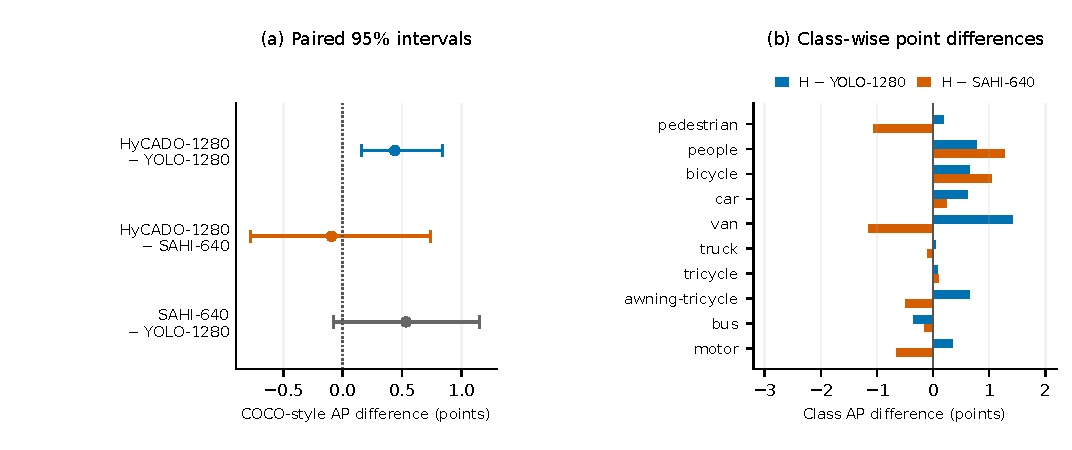
\includegraphics[width=\textwidth]{figures/coco_comparison.pdf}
\caption{Test-dev COCO-style comparisons at maxDets100. (a) Paired AP differences with marginal 95\% percentile intervals from 1000 draws over 61 filename/hash proxy groups. Positive differences favor the first named method. (b) Class-wise AP point differences, with H denoting HyCADO-1280; no class-specific intervals were computed. All comparisons condition on the retained trained models and the previously examined test-dev split.}
\label{fig:coco-comparison}
\end{figure*}

\subsection{Separating Proposal and Global-Detection Resolution}
The original cascade uses input target 800 for both proposal generation and global detections. The extension holds the crop network at $960\times960$ and changes these two YOLO roles. On all 647 internal-development images, regenerating regions at 1280 yields 32.410 toolkit AP versus 31.651 for YOLO-1280, a 0.758-point increment [0.472, 1.217]. Reapplying only final NMS to YOLO-1280 leaves 31.651 AP. The earlier replay retaining 800-based regions reaches 32.471 AP and uses 10682 crops rather than 11552.

On test-dev, retaining 800-based regions with 1280 global detections yields 24.469 COCO-style AP: $+0.473$ [0.199, 0.857] over YOLO-1280. HyCADO-1280 minus this variant is $-0.034$ [$-0.075$, $0.017$]. The analogous toolkit increments are 0.505 [0.129, 0.885] for HyCADO-1280 and 0.544 [0.168, 0.924] for the 800-region variant. The latter uses 25863 crop calls rather than 27682, about 6.6\% fewer. It also requires a separate 800-target YOLO proposal pass when the global output is computed at 1280; crop counts alone therefore do not establish a total-cost ordering. Both fixed variants are reported, rather than choosing a final method from their small observed difference. The missing 1280-proposal/800-global cell prevents a complete factorial analysis.

\subsection{Placement Controls and the Original Configuration}
Table~\ref{tab:accuracy} retains the historical VAL comparisons. HyCADO-800 reaches \APHybrid\ $\APlit$ versus \APYolo\ for YOLO-800, a \GainYolo-point difference. The relocation mean is 28.448, giving a \GainLocation-point placement margin. The individual relocation APs are 28.486, 28.407, and 28.451, with sample standard deviation 0.039 across the three position randomizations. The selected regions and their relocations share crop counts, ordered dimensions, detector weights, and fusion rules.

\begin{table*}[t]
\caption{Historical toolkit accuracy on all 548 VisDrone VAL images. SAHI suffixes give slice size. Relocation averages three separate placement scores. Macro AP is the equal-class toolkit diagnostic, distinct from COCO-style AP. HyCADO v1 denotes HyCADO-800.}
\label{tab:accuracy}
\centering\small\begin{tabular}{lrrrrr}
\toprule
Method & $\APlit$ & AP50 & AP75 & AR500 & Macro AP\\
\midrule
YOLOv9-C at 800 (YOLO-800) & 27.839 & 47.164 & 27.660 & 37.941 & 27.444\\
YOLOv9-C at 1280 (YOLO-1280) & 31.914 & 54.259 & 31.802 & 44.037 & 30.981\\
YOLOv9-C at 1536 (YOLO-1536) & 30.996 & 53.155 & 30.570 & 43.907 & 29.874\\
YOLOv9-C + SAHI-640 & 32.254 & 55.464 & 31.702 & 46.709 & 31.327\\
YOLOv9-C + SAHI-800 & 31.409 & 53.727 & 31.105 & 44.290 & 30.795\\
HyCADO v1 (YOLO-800 + crop RT-DETR-L) & 29.987 & 50.673 & 29.795 & 44.588 & 29.305\\
\midrule
Full-image RT-DETR-L & 19.760 & 37.474 & 18.110 & 29.559 & 18.730\\
Global fusion, $\alpha=1$ & 24.394 & 45.449 & 22.650 & 40.546 & 24.005\\
Global fusion, $\alpha=0.25$ & 29.316 & 50.251 & 28.791 & 41.820 & 28.849\\
Fixed grid + YOLO-800 & 28.810 & 48.732 & 28.598 & 41.573 & 28.130\\
Relocation mean (three placements) & 28.448 & 48.046 & 28.288 & 40.284 & 27.861\\
\bottomrule
\end{tabular}

\end{table*}

The equal-class toolkit diagnostic preserves the placement ordering: HyCADO reaches 29.305 versus 27.861 for the relocation mean. The fixed grid obtains 28.810 $\APlit$, 1.178 points below HyCADO, while using 5964 instead of 10057 crop calls. It therefore compares different placement, scale, coverage, and view budgets. Table~\ref{tab:ci} gives the paired placement and configuration intervals.

\begin{table}[t]
\caption{Historical VAL toolkit AP differences and marginal 95\% proxy-cluster bootstrap intervals, conditional on the retained models.}
\label{tab:ci}
\centering\small\begin{tabular}{lrrr}
\toprule
HyCADO v1 minus & $\Delta$AP & 95\% interval & Draws\\
\midrule
YOLO-800 & +2.148 & [1.915, 2.418] & 2000\\
Relocation mean & +1.539 & [1.373, 1.739] & 2000\\
Fixed grid & +1.178 & [0.994, 1.353] & 2000\\
Global fusion (0.25) & +0.671 & [0.486, 0.904] & 2000\\
YOLO-1280 & -1.927 & [-2.483, -1.222] & 1000\\
YOLO-1536 & -1.009 & [-1.884, -0.022] & 1000\\
SAHI-640 & -2.267 & [-3.041, -1.477] & 1000\\
SAHI-800 & -1.422 & [-1.979, -0.753] & 1000\\
\bottomrule
\end{tabular}

\end{table}

The placement result has the same direction on test-dev. HyCADO-800 reaches 26.768 toolkit AP, compared with 25.670 for YOLO-800 and relocation scores 25.630, 25.617, and 25.632. Its margin over the relocation mean is 1.142 points [0.792, 1.452], with the same 25863 ordered crop dimensions in each placement condition. The supplementary COCO evaluation gives HyCADO-800 22.377 AP versus relocation scores 21.428, 21.405, and 21.430; these are point comparisons without a new placement CI. The toolkit gain over YOLO-800 decreases from 2.148 points on VAL to 1.098 on test-dev, showing that the magnitude depends on the evaluated split even when the direction persists.

\subsection{Global Fusion, Resolution, and Slicing Controls}
Full-image fusion clarifies how much of the original detector comparison can arise from adding a second prediction source. A full-image RT-DETR multiplier of one gives \APGlobalRaw\ toolkit AP; transferring the crop multiplier of 0.25 gives \APGlobal\ AP. HyCADO-800 exceeds the latter by \GainGlobal\ points [0.486, 0.904]. The two RT-DETR models have different training views, so this comparison characterizes complete configurations rather than isolating crop placement alone.

Stronger uses of the same YOLO checkpoint also matter. On VAL, YOLO-1280 reaches \APYoloHigh\ toolkit AP, exceeding HyCADO-800 by \HighAPLead\ points. The paired HyCADO-minus-YOLO interval is [$-2.483$, $-1.222$]. YOLO-1536 also exceeds HyCADO-800 but falls slightly below YOLO-1280. SAHI-640 and SAHI-800 reach 32.254 and 31.409 toolkit AP. The COCO-style VAL evaluation preserves this broad ordering: 31.095 for YOLO-1280, 31.433 for SAHI-640, and 29.457 for HyCADO-800. These comparisons motivated the fixed 1280 cascade extension; they are retained alongside its results.

\subsection{Recall at Stated False-Positive Budgets}
For the final configuration, Figure~\ref{fig:recall-testdev} shows the full recorded test-dev recall--FP range, using a common horizontal scale that also resolves the low-FP region. At two false positives per image, YOLO-1280, HyCADO-1280, and the 800-region variant have the same observed recall: 32.690\% at IoU 0.50 and 22.402\% at IoU 0.75. The paired differences at this primary budget are zero in all 1000 draws. Point differences also equal zero at budgets 0.5, 1, 5, and 10. Thus the AP and AR100 increments do not translate into a recall gain at these operating points.

\begin{figure*}[t]
\centering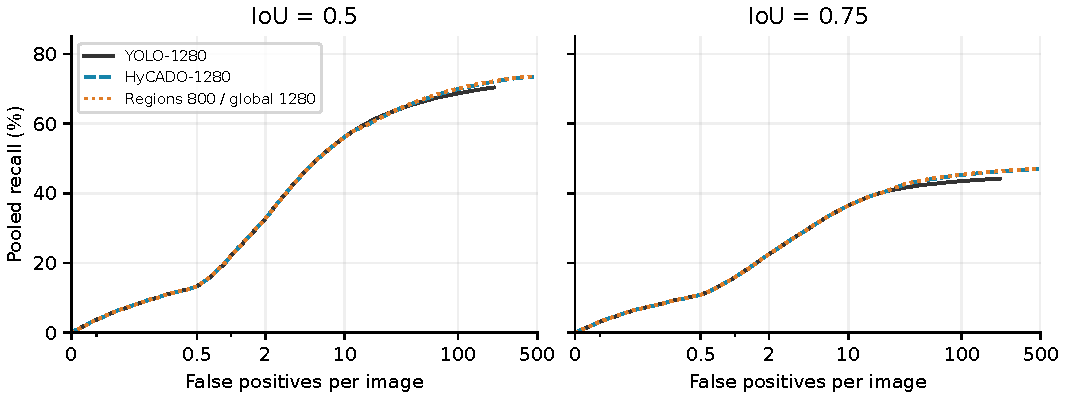
\includegraphics[width=.96\textwidth]{figures/recall_testdev_full_symlog.pdf}
\caption{Test-dev pooled recall versus false positives per image for frozen YOLO-1280 and the two refinement variants. Matching uses the toolkit-aligned global max500 prefix, not the COCO per-category cap. Whole score ties are retained. The horizontal axis is linear from zero to 0.5 FP/image and logarithmic above 0.5, with identical limits in both panels. Curves end at their actual archived-score coverage. The three methods coincide at the stated low-FP budgets; higher-FP differences are visible without artificial curve offsets. SAHI and two-resolution fusion were not included in this diagnostic.}
\label{fig:recall-testdev}
\end{figure*}

\begin{figure*}[t]
\centering\includegraphics[width=\textwidth]{figures/qualitative1280_main.pdf}
\caption{Fixed-sample qualitative comparison on VisDrone DET test-dev. Columns show GT, YOLO-1280, HyCADO-1280, and SAHI-640. Rows (a)--(c) are the first three images in a deterministic hash-ranked sample spanning distinct filename proxy groups. Every method shares the same native window and final-score display threshold of 0.05. Colors denote object classes; boxes are clipped only for display. The supplementary atlas contains all twelve sampled images and their context.}
\label{fig:qualitative}
\end{figure*}

The observed cutoffs at two false positives per image are 0.769 and 0.831 for the two IoUs, above the maximum scaled crop score of 0.25. At ten false positives per image the cutoffs remain 0.300 and 0.541. The unchanged high-score global prefix explains the observed overlap at these budgets; additional crop candidates enter the lower-score region. This connects the fusion rule to the operating-point results without treating a common score threshold as calibrated across detectors.

The earlier VAL diagnostic concerns HyCADO-800. At IoU 0.50 and two false positives per image, YOLO-1280 has 35.04\% recall and HyCADO-800 33.60\%. In the 99-image group with 1--30 normal objects the point estimates are 59.72\% and 62.30\%, respectively, with a difference interval spanning zero. At the original detection cap, larger-object recall improvements can coexist with substantially more false positives. The retained VAL size, object-count, and matched-budget tables provide the full historical breakdown in the supplement.

\subsection{Qualitative Comparison of the Final Configuration}
Figure~\ref{fig:qualitative} shows GT, YOLO-1280, HyCADO-1280, and SAHI-640 in identical native-pixel windows. The first three images of a fixed twelve-image hash-ranked sample form the main figure, with one image per distinct filename-based proxy group. Image selection was fixed before viewing these qualitative outputs and does not depend on model success. The test-dev split itself had already been examined in prior analyses. The supplementary qualitative atlas retains all twelve examples, their full-image context, and the selection record.

Each displayed $640\times420$ window maximizes the number of normal-GT centers among at most 100 deterministically spaced annotation-order candidates, with coordinate tie-breaking. This GT-based choice is used only for presentation. Frozen predictions are shown at score $\geq0.05$ after ignore-region preprocessing, without additional NMS or candidate truncation. Colors identify classes, not TP/FP status. Shared detections and changes in candidate extent and class assignment remain visible. The common numerical threshold neither calibrates the sources nor matches their false-positive rates; the examples complement the aggregate measurements rather than providing an additional accuracy estimate.



\subsection{Crop-Score Sensitivity and Matched Geometry}
Figure~\ref{fig:alpha} reports the complete five-point multiplier grid with the same trained models and regions. Overall COCO AP is 23.996 with the crop branch disabled, 24.510 at $\alpha=0.125$, 24.435 at 0.25, 24.189 at 0.5, and 22.256 at 1. The highest tested overall point estimate differs from the original multiplier by only 0.075 points; no interval was computed for that difference. It remains 0.802 points below two-resolution fusion. Small-object AP is highest in this grid at the original multiplier, 15.906, compared with 15.897 at 0.125. The $\alpha=0.25$ predictions and all retained COCO metrics reproduce the earlier result exactly. These observations describe sensitivity rather than selecting a new final multiplier on test-dev.

\begin{figure*}[t]
\centering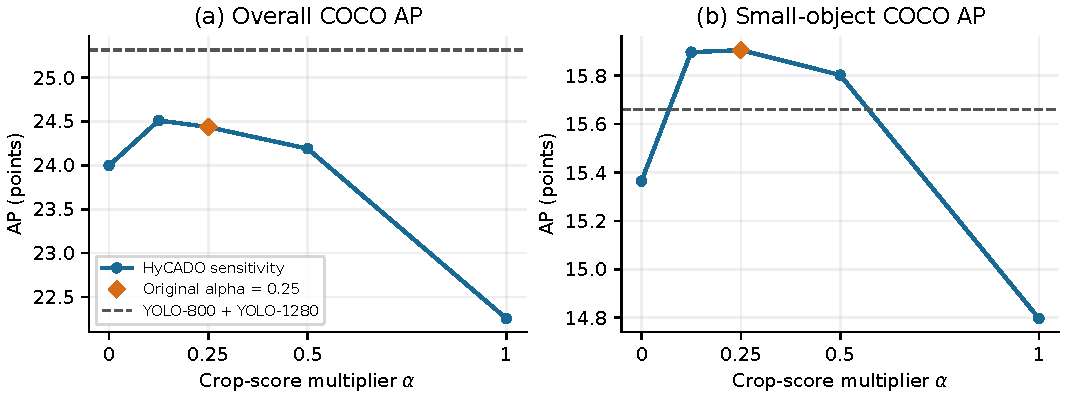
\includegraphics[width=\textwidth]{figures/alpha_sensitivity.pdf}
\caption{Descriptive test-dev multiplier sensitivity at maxDets100. (a) Overall AP. (b) Small-object AP. Zero disables the crop branch; positive values re-sort all candidates and rerun the unchanged final NMS. The original multiplier is highlighted. The dashed reference is two-resolution YOLO fusion. These are point estimates without new confidence intervals, not a held-out selection of an optimal multiplier.}
\label{fig:alpha}
\end{figure*}

The raw geometry audit finds that 4676 of 57341 retained crop boxes with display score at least 0.05 occupy at least 95\% of their crop area (8.155\%). After ignore preprocessing and the COCO per-class cap, 4534 such boxes remain in the evaluated display subset; all are counted as FP at both IoU 0.50 and 0.75. Across all evaluated crop boxes, including lower scores, the crop-filling subset has 2 TP and 8498 FP at IoU 0.50. FP here includes duplicate detections and class/localization errors under COCO's score-ordered matching; it is not a claim that every box is geometrically invalid. The measured pattern provides a specific diagnostic of the current crop outputs. No box-removal counterfactual was evaluated, so these counts do not quantify the AP effect of filtering that pattern. The supplement gives the full matched breakdown.

\subsection{Computation Budget}
Regional refinement adds one $960\times960$ crop-network pass per selected region. HyCADO-800 averages 18.35 crops on VAL and 16.06 on test-dev; HyCADO-1280 averages 17.19 on test-dev. The original sequential HyCADO-800 implementation averaged \HybridLatency\,ms/image in a warmed batch-one session on an RTX 3060 Ti. That historical measurement does not estimate either test-dev 1280 variant. The method trades additional detector passes and a second trained model for the reported accuracy increment; crop counts and input sizes make this budget explicit.

\section{Discussion and Limitations}
Three findings organize the evidence. First, selected crop locations contribute within the fixed cascade: the matched relocation margin remains positive on VAL and test-dev under the historical toolkit endpoint. Second, regional refinement adds accuracy over the single-resolution YOLO-1280 reference, with a small-object point advantage over the tested slicing and two-resolution comparators. Third, combining two global resolutions gives the highest overall AP among the evaluated configurations. The controlled comparisons distinguish a contribution within the cascade from superiority over alternative ways of using the same first-stage weights.

Proposal resolution and global prediction quality play distinct roles. Retaining the original 800-based regions gives a similar AP increment to regenerating them at 1280. This supports evaluating those two choices separately rather than assuming that more detailed proposals necessarily yield a better cascade. The point estimates also show smaller gains over stronger global predictions and a reduction in the original 800-cascade gain from VAL to test-dev. The benefit should therefore be interpreted for the stated models, split, and operating range.

The multiplier sensitivity and matched geometry explain two aspects of the score-fusion interface. Giving the raw crop scores full weight lowers overall AP, while the original attenuation preserves an increment over YOLO-1280. Crop-filling predictions supply a concrete FP pattern under the stated matching definition. Neither a multiplier sweep nor these counts establish a calibrated scoring rule or the benefit of a new geometry filter. The fusion multiplier also helps explain why additional candidate coverage need not improve high-confidence operation. Crop scores cannot exceed 0.25 after scaling, while the measured low-FP cutoffs remain higher. AP integrates over lower-score candidates as well; a positive AP increment and unchanged low-FP recall are consistent outcomes. A task that values these operating points differently may prefer a different complete inference configuration. No runtime improvement is inferred from the accuracy results.

The study has defined limits. It uses one dataset and one training seed; all bootstrap intervals describe sample-composition variation conditional on these models. Filename/hash groups are reproducible proxies, not verified independent scenes. Internal development and VAL had been examined before later controls, the 1280 extension followed the original test-dev analysis, and COCO, SAHI, two-resolution fusion, and score/geometry analyses followed earlier results. These extensions are exploratory and provide no new untouched confirmation set. Marginal secondary intervals are not multiplicity-adjusted; class and area results have no separate uncertainty estimates.

The controls also have bounded interpretations. Uniform relocation retains HyCADO's shapes and counts, while the crop model was trained on its selected views; it is not a comparison against a learned density or utility selector. Global fusion changes the RT-DETR training view, and there is no matched crop-trained same-family cascade to isolate detector-family diversity. YOLO-1280 reuses weights trained at target 800 rather than a separately optimized 1280 training recipe. Equal-compute retraining, selector sensitivity, alternative learned or calibrated fusion rules, and a complete resolution factorial remain outside the completed experiment set. The completed multiplier grid is descriptive and does not supply uncertainty across training seeds or a new untouched test. These limits define opportunities for subsequent work without changing the measured contribution of the current system.

\section{Conclusion}
HyCADO provides a reproducible setting for studying detector-guided regional refinement through placement, resolution, and score-fusion controls. Matched relocation supports a contribution from selected crop locations, and refinement added to YOLO-1280 yields a \CocoHY-point COCO-style AP increment on the evaluated test-dev split. Two-resolution YOLO fusion achieves a higher overall AP, while HyCADO-1280 retains a small-object point advantage over that comparator. Exact raw-query replay links the original result to a bounded multiplier sensitivity analysis and source-attributed crop-filling FP diagnostics. Together with the class-wise and operating-point evidence, these results show why the value of regional refinement depends on the alternative inference views, the object scales, and the ranking of additional predictions.

\section*{Data and Code Availability}
VisDrone data and the public evaluation toolkit are distributed by their maintainers~\cite{du2019visdrone,visdrone_toolkit}. The accompanying materials provide the manuscript source, recorded numerical evidence, paired-draw checks, fixed inference/evaluation packages, and qualitative selection records. The repository and immutable source snapshot are identified in the reproducibility subsection. Completed stages 22--25 and their numerical-source records are included in that public snapshot. The later completed 28--30 reports, fixed runnable packages, numerical checks, compiled figures, and image atlas accompany this revision. Public download locations for the trained checkpoints and complete frozen prediction databases remain pending.


\bibliographystyle{IEEEtran}
\bibliography{ref}
\end{document}
